\documentclass[serif]{beamer}

\mode<presentation>{
  \usetheme{Pittsburgh}
%--------------------------------------------------
%   \setbeamercovered{transparent}
%-------------------------------------------------- 
  \setbeamerfont{institute}{size=\normalsize}
  \setbeamerfont{section in toc}{size=\large}
  \setbeamerfont{subsection in toc}{size=\normalsize}
  \setbeamertemplate{frametitle}{%
    \vskip 12pt
    \begin{centering}
    \structure{\textbf{\insertframetitle}}\par
    \end{centering}
  }
}

\usepackage[english]{babel}
\usepackage{times}
\usepackage{algorithmic}
\usepackage{algorithm}
\usepackage{epsfig}
\usepackage{pgf}
\usepackage[absolute,overlay]{textpos}

\usepackage{pst-all} % PSTricks
\usepackage{com.braju.graphicalmodels} % The package that really does the hard work

%--------------------------------------------------
% \usepackage{mathtime}
%-------------------------------------------------- 

% Latin-1 only
\usepackage[latin1]{inputenc}
\usepackage[T1]{fontenc}
%--------------------------------------------------
% % Chinese-support
% \usepackage[nocjkbg5]{ucs}
% \usepackage[utf8x]{inputenc}
% \usepackage[C00,T1]{fontenc}
% \newcommand\tradtext[1]{\bgroup\fontencoding{C00}\fontfamily{ming}\selectfont%
% \SetUnicodeOption{cjkbg5}#1\egroup}
%-------------------------------------------------- 

\title[]{Multiple-Representation Relevance Model}
\author[]{Ruey-Cheng Chen <cobain@turing.csie.ntu.edu.tw>}
\institute{National Taiwan University, Taiwan}
\date[]{\today}
\subject{Information Retrieval}
%--------------------------------------------------
% \AtBeginSubsection[]
% {
%   \begin{frame}<beamer>
%     \frametitle{Outline}
%     \tableofcontents[currentsection,currentsubsection]
%   \end{frame}
% }
%-------------------------------------------------- 
%\beamerdefaultoverlayspecification{<+->}
\newcommand<>\ul[2]{\textbf{#1}\begin{itemize}#2\end{itemize} \vskip 0.5em}
\newcommand<>\ull[1]{\begin{itemize}#1\end{itemize}}
\newcommand<>\ol[2]{\textbf{#1}\begin{enumerate}#2\end{enumerate}}
\newcommand<>\oll[1]{\begin{enumerate}#1\end{enumerate}}
\newcommand<>\dl[2]{\textbf{#1}\begin{description}#2\end{description}}
\newcommand<>\f[2]{\begin{frame}{#1}#2\end{frame}}
\newcommand<>\mydef[2][]{\textbf{#1}\par#2\par}
\newcommand<>\tbl[3]{\textbf{#1}\vskip 0.5em\begin{center}\begin{tabular}{#2}#3\end{tabular}\end{center}}
\newcommand<>\fig[3]{\textbf{#1}\vskip 0.5em\begin{center}\begin{figure}\includegraphics[#2]{#3}\end{figure}\end{center}}
\newcommand<>\cols[1]{\begin{columns}#1\end{columns}}
\newcommand<>\col[2]{\begin{column}{#1}#2\end{column}}

\begin{document}

\frame{ \titlepage }

%--------------------------------------------------
% \f{References}{
%   \ul{Mandatory References}{ 
%     \item Craswell, N. and Szummer, M. 2007. Random walks on the click graph.
%     In \emph{Proceedings of the 30th Annual international ACM SIGIR Conference
%     on Research and Development in information Retrieval} (Amsterdam, The
%     Netherlands, July 23 - 27, 2007). SIGIR '07. ACM, New York, NY, 239-246.
%   }
% 
%   \ul{Authors}{ 
%     \item Nick Craswell: \footnotesize{\url{ http://research.microsoft.com/~nickcr/ }}
%     \item Martin Szummer: \footnotesize{\url{ http://research.microsoft.com/~szummer/ }}
%   }
% }
%-------------------------------------------------- 

\f{Outline}{ \tableofcontents }

\section{Introduction}
\f{Document Representation}{
  \ul{In conventional thinking...}{
    \item We assume a document is represented as a collection of term
    \item A more subtle assumption: Every document possesses \textbf{only one} such representation
    \item This leads to simple, effective retrieval models, such as: \ull{
      \item Vector-space model
      \item Binary-independence retrieval model
      \item Language modeling approach
    }
  }

  \ul{The downside}{
    \item Terms are supposed to be homogeneous (or drawn from a mixture of homogeneous data sources)
    \item There is no room for modeling user-contributed tags, annotations, and metadata
  }
}

\f{Multi-Layer Document Representation}{
  \ul{Information sources relevant to a document}{
    \item Metadata: Precise, detailed descriptions 
    \item Tags: Short, less precise, conceptual descriptions
    \item Fulltext: Long and loose text; diverse vocabulary
  }

  \ul{We need additional layers in a retrieval model because...}{
    \item Incorporation of vocabularies enables high usability
    \item Retrieval can then be operated in different granularity levels
    \item Retrieval can be operated on a mixture of \textbf{heterogeneous} sources
    \item Possible applications include...
    \ull{
      \item Cross-language query modeling 
      \item Cross-vocabulary query modeling
      \item Named-entities ranking
    }
  }
}

\f{Challenge: Building the Model}{
  \ul{A language model that work with two document representation}{
    \item \emph{Terms} are denoted as $T$
    \item The \emph{secondary document representation} is denoted as $S$
    \item We built a model to enable interaction between the two layers, such as 
    retrieving elements in one side from that in the other
  }

  \mydef[Formulation]{
    We want to estimate the probability $\Pr(s|t)$, given that a document $d_i$
    is indexed in two different representations $T_i$ and $S_i$, where $T_i
    \subset T$ and $S_i \subset S$.  A concrete application of this is to let
    the user form a query $\mathbf{q} \subset T$ and estimate the probability
    $\Pr(s|\mathbf{q})$ accordingly.
  }
}

\f{Roadmap}{
  \ul{Where do we go from here?}{
    \item We proposed a generalization over Lavrenko and Croft's work \cite{lavrenko2001relevance} by
    adapting it to cases where two document representations are appropriate
    \item We took a Bayesian generative approach 
    \item The result can be easily implemented in index level
    \item Two applications are introduced to evaluate our work 
    \ull{ \item Refining query model by using secondary representation \item Retrieving query-dependent facets }
    \item The model achieved satisfactory result in both experiments
  }
}

\section{Related Work}

\f{Related Work}{
  \ul{Query modeling}{
    \item Our method was inspired by the recent advances on language modeling
    applications \cite{lavrenko2001relevance,zhai2001language,zaragorza2003bayesian}
    \item Our approach differs from the previous work in the presence of a secondary document representation
  }
  \par
  \ul{Facet ranking}{
    \item Our work is among the earliest attempt for facet ranking
    \item Similar attempts were made in the area of expert finding \ull{
      \item Amitay et al. \cite{amitay2008finding} formulated the problem of expert
      finding as a two-layered retrieval task by using \emph{inverse entity-frequency} 
      \item Balog et al. \cite{balog2009language} followed up and
      proposed a language modeling approach with the similar rationale to
      exploit person-term and person-document links
    }
    \item Our approach departs from these work in the 
    way document relevance is modeled and that prior belief is supported
  }
}

\section{Model}
\subsection{The Generative Framework}

\f{The Generative Framework}{
  \begin{figure}
    \centering
    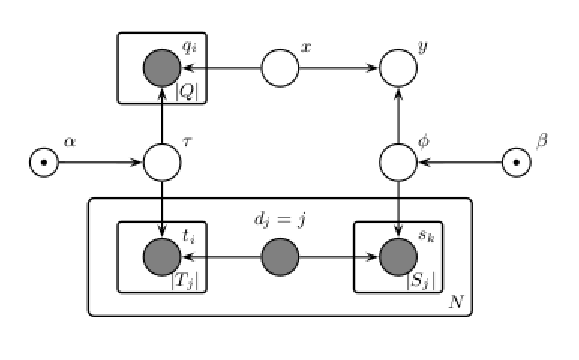
\includegraphics[width=8cm]{model}
  \end{figure}

  \ul{Tips for reading the plate notations}{

    \only<1>{ \item Circles are variables; observed variables are shaded.
    \item Dotted circles denotes hyperparameters.  \item Arrows denote
    dependencies. }

    \only<2>{ \item Consider the collection is composed of $N$ documents.
    \item Each document $d_j$ is associated with two sets of terms $T_j$ and
    $S_j$. \item We refer $T_j$ as the primary representation and $S_j$ as the
    secondary. }
    
    \only<3>{ \item Each document $d_j$ possesses two multinomials $\tau^{(j)}$
    and $\phi^{(j)}$ from which elements in $T_j$ and $S_j$ are drawn,
    respectively.  \item Now we have two document models $p(w|\tau^{(j)})$ and
    $p(w|\phi^{(j)})$. }

    \only<4>{ 
      \item The multinomils work on two different sets of vocabularies.
      \item Two Dirichlets $\{\alpha_i; i \in [1, |T|]\}$ and $\{\beta_k; k \in [1, |S|]\}$ are assumed. 
      \item They govern the generation of the document multinomials.
    }
  }
}

\f{The Generative Framework}{
  \begin{figure}
    \centering
    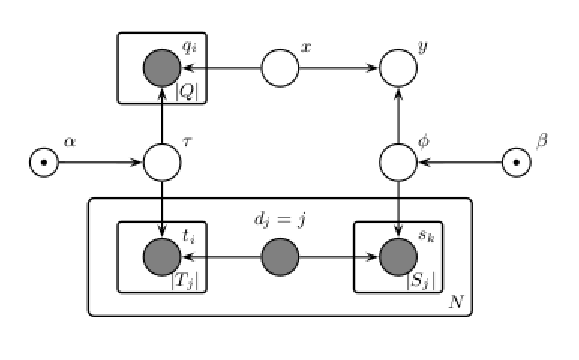
\includegraphics[width=8cm]{model}
  \end{figure}

  \mydef[Obtaining the predictive distribution]{

    \only<1>{The query $\mathbf{q}$ is a set of observed terms drawn
    from an unknown document model $x$ in the collection.  Specifically, the
    query terms are encoded in the same vocabulary as in that form the primary
    representation of document $x$.}
    
    \only<2>{By making this assumption, we are able to match the query
    against all the document models and to estimate the query likelihood
    $\Pr(\mathbf{q}|d_j)$.  This leads us to the probabilistic generative methods,
    such as language modeling.}
    
    \only<3>{Recall that the unknown document $x$ is connected
    to another unknown variable $y$.  The variable $y$ represents the most probable
    term generated from the secondary multinomial distribution $\phi^{(x)}$.}

  }
}

\f{Summary of the Framework}{
  \mydef[]{
    The entire generative process can be summarized as follows:
    \begin{enumerate} 
      \item For each document $d_j$, \begin{enumerate}
	\item $\tau^{(j)} \sim \textrm{Dirichlet}(\alpha_i; i \in [1, |T|])$
	\item $\phi^{(j)} \sim \textrm{Dirichlet}(\beta_k; i \in [1, |S|])$
	\item For $i \in \{ 1, \ldots, |T_j| \}$, $t_i \sim \textrm{Mult}(\tau^{(j)})$ 
	\item For $k \in \{ 1, \ldots, |S_j| \}$, $s_k \sim \textrm{Mult}(\phi^{(j)})$ 
      \end{enumerate}
      \item For some unknown document $d_x$, \begin{enumerate}
	\item For $i \in \{ 1, \ldots, |\mathbf{q}|\}$, $q_i \sim \textrm{Mult}(\tau^{(x)})$
      \end{enumerate}
    \end{enumerate}
  }
}

\subsection{Inference}

\f{Term Likelihood in the Second Representation}{
  \mydef[Formulation]{
    We want to explicitly estimate the likelihood of one term $s$ in the
    secondary term domain being ``\emph{triggered}'' by another set of terms
    from the primary term domain.  This task can be framed as a optimization
    problem: \begin{equation} y^* = \arg\max_{y \in S} \Pr(y|\mathbf{q},
    \mathbf{t}, \mathbf{d}, \mathbf{s}) \label{eq:forward} \end{equation} where
    $\mathbf{t}$ and $\mathbf{s}$ represent all the observed terms in the
    primary/secondary representations in the collection, respectively;
    $\mathbf{q}$ represents the input query and $\mathbf{d}$ denotes all the
    observed documents.  
  }
}

\f{Inference (For Impatient Readers)}{
  \begin{eqnarray}
    \Pr(y|\mathbf{q}, \mathbf{t}, \mathbf{d}, \mathbf{s}) 
    &=& \sum_{x \in [1, N]} \Pr(y|x, \mathbf{q}, \mathbf{t}, \mathbf{d}, \mathbf{s}) \Pr(x|\mathbf{q}, \mathbf{t}, \mathbf{d}, \mathbf{s}) \nonumber\\
    &\propto& \sum_{x \in [1, N]} \left\{ \int \Pr(y|x, \phi^{(x)}) \Pr(\phi^{(x)}|d_x, \mathbf{s_x}) \mathrm{d}\phi^{(x)} \right. \nonumber\\
    && \left. \int \Pr(\mathbf{q}| x, \tau^{(x)}) \Pr(\tau^{(x)}|d_x, \mathbf{t_x})\mathrm{d}\tau^{(x)} \Pr(x) \right\} \nonumber\\
    &=& \alert{\sum_{x \in [1, N]} \frac{\beta_y + c_{y,x}}{\sum_k \beta_k + c_{k,x}} \frac{\mathcal{B}(\{\alpha_i + c_{i,x} + c_{i,q} \})}{\mathcal{B}(\{\alpha_i + c_{i,x} \})} \Pr(x)} \label{eq:forward-solution}
  \end{eqnarray}
  Recall that $\mathcal{B}(\cdot)$ is the multinomial beta
  function defined by \[\mathcal{B}(a_1, \ldots, a_n) = \frac{\prod_i
  \Gamma(a_i)}{\Gamma(\sum_i a_i)}. \]
}

\f{Inference: Step by Step}{
  \mydef[Inducing the first term in the summation]{
    \begin{eqnarray}
      \Pr(y|\mathbf{q}, \mathbf{t}, \mathbf{d}, \mathbf{s}) &=& \sum_{x \in
      [1, N]} \alert{\Pr(y|x, \mathbf{q}, \mathbf{t}, \mathbf{d}, \mathbf{s})}
      \Pr(x|\mathbf{q}, \mathbf{t}, \mathbf{d}, \mathbf{s}) \nonumber\\
      && \nonumber\\
      \Pr(y|x, \mathbf{q}, \mathbf{t}, \mathbf{d}, \mathbf{s})
      &=& \int \Pr(y, \phi^{(x)}|x, \mathbf{q}, \mathbf{t}, \mathbf{d}, \mathbf{s}) \mathrm{d}\phi^{(x)} \nonumber\\
      &=& \int \Pr(y|\phi^{(x)}, x, \mathbf{q}, \mathbf{t}, \mathbf{d}, \mathbf{s}) 
      \Pr(\phi^{(x)}|x, \mathbf{q}, \mathbf{t}, \mathbf{d}, \mathbf{s}) \mathrm{d}\phi^{(x)} \nonumber\\
      &=& \int \Pr(y|\phi^{(x)}, x) \Pr(\phi^{(x)}|d_x, \mathbf{s}_x) \mathrm{d}\phi^{(x)} \label{eq:first}
    \end{eqnarray}
  }
}

\f{Inference: Step by Step}{
  \mydef[Inducing the second term in the summation]{
    \begin{eqnarray}
      \Pr(y|\mathbf{q}, \mathbf{t}, \mathbf{d}, \mathbf{s}) &=& \sum_{x \in
      [1, N]} \Pr(y|x, \mathbf{q}, \mathbf{t}, \mathbf{d}, \mathbf{s})
      \alert{\Pr(x|\mathbf{q}, \mathbf{t}, \mathbf{d}, \mathbf{s})} \nonumber\\
      && \nonumber\\
      \Pr(x|\mathbf{q}, \mathbf{t}, \mathbf{d}, \mathbf{s})
      &=& \frac{\Pr(\mathbf{q}|x, \mathbf{t}, \mathbf{d}, \mathbf{s}) \Pr(x|\mathbf{t}, \mathbf{d}, \mathbf{s})}
      {\Pr(\mathbf{q}|\mathbf{t}, \mathbf{d}, \mathbf{s})} \nonumber\\
      &\propto& \Pr(\mathbf{q}|x, \mathbf{t}, \mathbf{d}, \mathbf{s}) \Pr(x|\mathbf{t}, \mathbf{d}, \mathbf{s}) \nonumber\\
      &=& \left( \int \Pr(\mathbf{q}, \tau^{(x)}|x, \mathbf{t}, \mathbf{d}, \mathbf{s}) \mathrm{d}\tau^{(x)} \right) 
      \Pr(x|\mathbf{t}, \mathbf{d}, \mathbf{s}) \nonumber\\
      &=& \left( \int \Pr(\mathbf{q}|\tau^{(x)}, x, \mathbf{t}, \mathbf{d}, \mathbf{s}) 
      \Pr(\tau^{(x)}|x, \mathbf{t}, \mathbf{d}, \mathbf{s}) \mathrm{d}\tau^{(x)} \right) 
      \Pr(x|\mathbf{t}, \mathbf{d}, \mathbf{s}) \nonumber\\
      &=& \int \Pr(\mathbf{q}|\tau^{(x)}, x) \Pr(\tau^{(x)}|d_x, \mathbf{t}_x) \mathrm{d}\tau^{(x)} \Pr(x) \label{eq:second}
    \end{eqnarray}
  }
}

\f{Inference: Step by Step}{
  \ul{Conjugate priors}{
    \item In Bayesian theory, the prior $\Pr(\theta)$ and posterior $\Pr(\theta|x)$
    are called conjugate distributions, if the posterior are in the same family as the prior
    \item Usually, it can be viewed as updating the prior belief on
    $\theta$ after observing a sequence of outcome $x$.
    \item Conjugate prior is an algebraically ``syntactic sugar'' to simplify inference
    \item Fast fact: Dirichlets are conjugate to multinomials \ull{
      \item $\Pr(\phi^{(x)}|x, y, d_x, \mathbf{s}_x) \sim \mathrm{Dirichlet}(\{\beta_k + c_{k,x}; \forall k\})$
      \item $\Pr(\tau^{(x)}|x, \mathbf{q}, d_x, \mathbf{t}_x) \sim \mathrm{Dirichlet}(\{\alpha_i + c_{i,x} + c_{i,q}; \forall i\})$
    }
  }
  \par
  \ul{Care for going into details?}{
    \item Detailed derivation is too terrifying/boring to be presented here
    \item Check out Gelman et al. for good reference on Bayesian statistics
  }
}

\f{Inference: Revisited}{
  \mydef[Integrating out the prior]{
    \begin{eqnarray}
    \int \Pr(y|x, \phi^{(x)}) \Pr(\phi^{(x)}|d_x, \mathbf{s_x}) \mathrm{d}\phi^{(x)} 
    &=& \frac{\beta_y + c_{y,x}}{\sum_k \beta_k + c_{k,x}} \\
    \int \Pr(\mathbf{q}| x, \tau^{(x)}) \Pr(\tau^{(x)}|d_x, \mathbf{t_x})\mathrm{d}\tau^{(x)} 
    &=& \frac{\mathcal{B}(\{\alpha_i + c_{i,x} + c_{i,q} \})}{\mathcal{B}(\{\alpha_i + c_{i,x} \})} 
    \end{eqnarray}
  }
  \par
  \mydef[Voila!]{
    \begin{eqnarray}
      \Pr(y|\mathbf{q}, \mathbf{t}, \mathbf{d}, \mathbf{s}) 
      &=& \sum_{x \in [1, N]} \Pr(y|x, \mathbf{q}, \mathbf{t}, \mathbf{d}, \mathbf{s}) \Pr(x|\mathbf{q}, \mathbf{t}, \mathbf{d}, \mathbf{s}) \nonumber\\
      &\propto& \alert{\sum_{x \in [1, N]} \frac{\beta_y + c_{y,x}}{\sum_k \beta_k + c_{k,x}} \frac{\mathcal{B}(\{\alpha_i + c_{i,x} + c_{i,q} \})}{\mathcal{B}(\{\alpha_i + c_{i,x} \})} \Pr(x)} \label{eq:forward-solution}
    \end{eqnarray}
  }
}

%--------------------------------------------------
%     \item For example, Dirichlets are conjugate to multinomials 
%     \item $\Pr(\phi^{(x)}|x, y, d_x, \mathbf{s}_x) \sim \mathrm{Dirichlet}(\{\beta_k + c_{k,x}; \forall k\})$
%     \item $\Pr(\tau^{(x)}|x, \mathbf{q}, d_x, \mathbf{t}_x) \sim \mathrm{Dirichlet}(\{\alpha_i + c_{i,x} + c_{i,q}; \forall i\})$
%-------------------------------------------------- 
}

\subsection{Hyperparameters and the Index Structure}

\f{Hyperparameters}{
  \ul{Prior distributions}{
    \item Prior represents our belief on the distribution of the model parameters
    \item General form: $(\beta_1, \beta_2, \ldots, \beta_{|S|})$
  }
  \par

  \ul{Uniform prior}{ \item $(c, c, \ldots, c)$ \item We let $\beta_k = c$ for
  each $k \in [1, |S|]$ and $c$ denote some constant }

  \ul{Smoothed-Dirichlet}{
    \item $(\mu \Pr(s_1|C), \mu \Pr(s_2|C), \ldots, \mu \Pr(s_{|S|}|C))$ 
    \item $\Pr(s_k|C)$ denotes the probability of generating term $s_k$ (in the secondary
term domain) from the collection by viewing the entire collection as one language model
    \item $\mu$ represents some constant.
    \item Widely-used as a smoothing method in the language modeling applications for information retrieval \cite{zhai2004study}
  }
}

\f{Index Structure}{
  \ul{Integration with the language model}{
    \item One interesting feature of our model is the seamless integration
    with the language-model-based retrieval method
    \item It comes from
    the fact we could further simplify Equations~\eqref{eq:forward-solution} by
    assigning $\alpha$ as a smoothed-Dirichlet prior and $\Pr(x)$ as a uniform
    prior
    \item When $\alpha_i = \mu \Pr(t_i|C)$, it can be shown that: \[
    \frac{\mathcal{B}(\{\alpha_i + c_{i,x} + c_{i,q} \})}{\mathcal{B}(\{\alpha_i +
    c_{i,x} \})} \propto {\rm L}_{\rm LM}(\mathbf{q}|d), \] where ${\rm L}_{\rm
    LM}(\mathbf{q}|d)$ denotes the query likelihood score in the language model
    with Dirichlet smoothing scheme
    
    \item In this case, the model scores becomes:
    \begin{eqnarray}
      \Pr(y|\mathbf{q}, \mathbf{t}, \mathbf{d}, \mathbf{s}) &\propto& 
      \alert{\sum_{x \in [1, N]} \frac{\beta_y + c_{y,x}}{\sum_k \beta_k + c_{k,x}}
      {\rm L}_{\rm LM}(\mathbf{q}|x)}
    \end{eqnarray} 
  }
}


\section{Experimental Results}
\subsection{Query Refinement Using the Secondary Representation}

\f{Query Refinement Using the Secondary Representation}{
  \ul{Idea}{
    \item Make an initial retrieval run
    \item Use the retrieved result to populate the refined model
    \item Re-submit the model as a new query
  }
  \par
  \ul{Why employing two-stage retrieval?}{
    \item $\Pr(y|\mathbf{q}, \mathbf{t}, \mathbf{d}, \mathbf{s})$ can be seen as a refined query model
    \item This technique was proposed in Lavrenko's work
    \item The new model is refined in the secondary representation
    \item The benefit of such a two-stage setup: \ull{
      \item The first run is done in general language (good for recall)
      \item The second run is done in specific language (good for precision)
    }
  }
}

\f{Query Refinement Using the Secondary Representation}{
  \ul{Facilatating the second-run retrieval}{
    \item The refined model is a probability distribution
    \item For each $s_k$, we calculated its \emph{expectation} $E(s_k|\mathbf{q}, \mathbf{t}, \mathbf{d}, \mathbf{s})$
    \item The expectation can be seen as the number of occurrence for $s_k$
    \item The resulting language model is: \[
      x^{*} &=& \arg\max_x \prod_k \Pr(s_k|x)^{E(s_k|\mathbf{q}, \mathbf{t}, \mathbf{d}, \mathbf{s})}
    \]
    \item This simple technique reduces to KL-divergence retrieval framework \cite{zhai2001language}
  }
}

\f{Evaluation}{
  \ul{Setup}{
    \item Task: Chinese-to-Chinese monolingual document retrieval
    \item The benchmark is available as part of NTCIR-4 Test Collection CLIR Task
    \item 381,681 newswire articles and 59 test topics were involved
    \item We used only title queries in the experiment 
    \item Primary representation: CJK-character bigrams + English word unigrams
    \item Secondary representation: High-discriminative CJK-character bigrams \ull{
      \item I.e., top-500,000 CJK-character bigrams ranked by tf-idf scores
      \item The minimum support for each bigram was 5
      \item The number (500,000) was determined through experimentation
    }
  }
}

\f{Evaluation}{
  \ul{Baseline methods}{
    \item We used the Lemur toolkit to build up strong baselines
    \item Participating runs include tf-idf, okapi, and indri (a language-model variant)
    \item Query refinement/expansion for each run: \ull{
      \item tf-idf: pseudo relevance-feedback
      \item okapi: pseudo relevance-feedback
      \item indri: adapted relevance model
    }
    \item The number of feedback documents: 20
    \item The number of feedback terms: 100
    \item Our refined model was truncated (preserving only top-100's)
    \item Performance was measured in terms of mean average-precision and precision-at-5
  }
}

\f{Evaluation Result}{
  \begin{table}[ht!]
    \scriptsize
    \centering
    \begin{tabular}{lllll}
      Method & MAP (+\%) & P@5 (+\%) & MAP (+\%) & P@5 (+\%) \\
      \hline
      {\tt tfidf} & 0.181 & 0.264 & 0.213 & 0.335 \\
      {\tt tfidf} + PRF & 0.217 (+19.9\%) & 0.295 (+11.7\%) & 0.264 (+23.9\%) & 0.383 (+14.3\%) \\
      {\tt okapi} & 0.185 & 0.278 & 0.223 & 0.356 \\
      {\tt okapi} + PRF & 0.224$^{**}$ (+21.1\%) & 0.315 (+13.3\%) & 0.270$^{**}$ (+21.1\%) & 0.400 (+12.4\%) \\
      \hline
      {\tt indri} & 0.174 & 0.258 & 0.216 & 0.346 \\
      {\tt indri} + Relevance & 0.180 (+3.4\%) & 0.271 (+5.3\%) & 0.222 (+2.8\%) & 0.342 (-1.2\%) \\
      {\tt lm} & 0.170 & 0.251 & 0.209 & 0.322 \\
      {\tt lm} + Refinement & 0.207$^*$ (+21.8\%) & 0.302 (+20.3\%) & 0.261$^*$ (+24.9\%) & 0.369 (+14.6\%) \\
      \\
    \end{tabular}

    \caption{The result for the query refinement task.  Retrieval methods listed in the
    upper-half are tfidf-based, while those in the lower-half are
    language-model-based.  The overall top-performer is indicated with two
    asterisks in the superscript, while the best run in the language-modeling
    side is indicated with one asterisk.}
    \label{t:query-modeling}
  \end{table}
}

\subsection{Retrieving Query-Relevant Facets}

\f{Retrieving Query-Relevant Facets}{
  \ul{Faceted search as a two-phase extension of the ordinary retrieval}{
    \item See \cite{hearst2002finding,yee2003faceted,roy2008minimum} for detail about faceted search
    \item One populates a set of documents by submitting the query
    \item One discovers facets by exploiting the associations between facets and documents 
    \item How do we present the facets?
  }
  \par
  \ul{Count-based presentation schemes}{
    \item Facets are sorted in descending order of the number of counts
    \item It is easy to implement (one more pass through the forward index)
    \item It treats all the facet count as equally importatnt \ull{
      \item e.g., A facet count in document #1 is as good as in document #100
    }
    \item Critics #1: It disregards the notion of relevance
    \item Critics #2: Users can be mislead when consulting the results to guide the subsequence exploratory search
  }
}

\f{Retrieval Query-Relevant Facets}{
  \ul{Idea}{
    \item Encode facets in the secondary representations of the corresponding associated documents
    \item Run the proposed model
  }
  \par
  \ul{Why using the secondary representation?}{
    \item This task is relevant to (but not equivalent to) expert finding 
    \item Use $\Pr(y|\mathbf{q}, \mathbf{t}, \mathbf{d}, \mathbf{s})$ to sort the facets
    \item Consider this method as a relevance-weighted version of the count-based approach
    \item It is efficient: fast as ad-hoc retrieval (with a little overhead forwarding scores)
  }
}

\f{Evaluation}{
  \ul{Setup}{
    \item Task: Retrieving relevant facets on Tan-Hsin Corpus
    \item The test data comprises 15,314 historical documents, each with person name facets
    \item 105 query topics are collected from the query logs 
    \item 28 topics were randomly selected and used in the experiment
    \item Relevance judgment was manually made for all the top 100 facets returned by the baseline retreiver
  }
  \par
  \ul{Methods}{
    \item \texttt{baseline}: The count-based scheme
    \item \texttt{uniform-prior}: The proposed method, using uniform prior for $\beta$
    \item \texttt{smoothed-prior}: The proposed method, using Dirichlet-smoothed prior for $\beta$
  }
}

\f{Evaluation Result}{
  \begin{table}[ht!]
    \centering
    \begin{tabular}{llll}
      Method & & MAP & P@10 \\
      \hline
      {\tt baseline} & & 0.2996 & 0.3857 \\
      {\tt uniform-prior} & $\beta = 0$ & 0.5775 & 0.6179\\
      & $\beta = 1$ & 0.5899$^*$ & 0.6464$^*$ \\
      & $\beta = 10$ & 0.5877 & 0.6464$^*$ \\
      {\tt smoothed-prior} & $\mu = 0.01$ & 0.5781 & 0.6179 \\
      & $\mu = 1$ & 0.5782 & 0.6214 \\
      & $\mu = 100$ & 0.4956 & 0.5429 \\
      \\
    \end{tabular}
    \caption{The performance results for all the test runs.  The top-performer is indicated by an asterisk in the superscript.}
    \label{t:performance}
  \end{table}
}

\section{Discussion and Concluding Remarks}
\f{Discussion and Concluding Remarks}{
  \ul{Our proposed framework...}{
    \item Enables the use of a secondary document representation in language modeling
    \item Offers interoperability between two different term domains
    \item Exploits the index structure to achieve high efficiency
  }

  \ul{Evaluation results}{
    \item Two applications were introduced in this work
    \item In the first task, the model beaten the relevance model baseline by 17.6\% (rigid) and 22.7\% (relax) in 
    MAP \ull{ 
      \item It achieved comparable performance as {\tt tfidf} with pseudo-relevance feedback
      \item The model alone improved the MAP of the regular language modeling run by 21.8\% (rigid) and 24.9\% (relax)
    }
    \item In the second application, the baseline performance was improved by
    roughly 100\% in MAP.  
  }
}

%--------------------------------------------------
% \section{Background}
% \subsection{Graph-Theoretical Concepts}
% \f{Graph}{
%   \ul{Basic Concepts}{
%     \item An undirected graph $G = (V, E)$ is a collection of nodes $V$ and edges $E$.
%     \item Two nodes $i, j \in V$ are \emph{neighbors} if $(i, j) \in E$.
%     \item Neighborhood of a node $i$: $\{j \mid (i, j) \in E\}$.
%     \item A node is not a neighbor of itself, i.e., $(i, i) \notin E$.
%     \item A clique of $G$ is either a single node or a complete subgraph of $G$.
%   }
%   \begin{figure}
%     \centering
%     \includegraphics[width=100pt]{clique}
%   \end{figure}
% }
% 
% \subsection{Random Fields}
% \f{Random Fields}{
%   \mydef[Random Fields]{
%     Let $F = \{X_1, \ldots, X_m\}$ be a set of random variables defined on the
%     sample space $\Omega$, in which each $X_i$ takes a value $x_i \in
%     \mathcal{L}$.  A probability measure $p$ is a \emph{random field} if
%     $p(\omega) > 0$ for all $\omega \in \Omega$.
%   }
%   \vskip1em
%   \ul{Random Fields on $G$}{
%     \item Assign each random variable $X_i$ to a node of $G$.
%     \item Values of random variables are usually spatially correlated.
%   }
%   \begin{figure}
%     \centering
%     \includegraphics[width=100pt]{rf}
%   \end{figure}
% }
%-------------------------------------------------- 
\section<presentation>*{\appendixname}

\begin{frame}[allowframebreaks]
  \frametitle{References}
  \small
  \bibliography{report}
  \bibliographystyle{alpha}
\end{frame}

\frame{
  \begin{center}
    \Huge{Thanks for your attention!}
    \par
    Any Question?
  \end{center}
}

\end{document}
